% Options for packages loaded elsewhere
\PassOptionsToPackage{unicode}{hyperref}
\PassOptionsToPackage{hyphens}{url}
\PassOptionsToPackage{dvipsnames,svgnames,x11names}{xcolor}
%
\documentclass[
  letterpaper,
  DIV=11,
  numbers=noendperiod]{scrartcl}

\usepackage{amsmath,amssymb}
\usepackage{iftex}
\ifPDFTeX
  \usepackage[T1]{fontenc}
  \usepackage[utf8]{inputenc}
  \usepackage{textcomp} % provide euro and other symbols
\else % if luatex or xetex
  \usepackage{unicode-math}
  \defaultfontfeatures{Scale=MatchLowercase}
  \defaultfontfeatures[\rmfamily]{Ligatures=TeX,Scale=1}
\fi
\usepackage{lmodern}
\ifPDFTeX\else  
    % xetex/luatex font selection
\fi
% Use upquote if available, for straight quotes in verbatim environments
\IfFileExists{upquote.sty}{\usepackage{upquote}}{}
\IfFileExists{microtype.sty}{% use microtype if available
  \usepackage[]{microtype}
  \UseMicrotypeSet[protrusion]{basicmath} % disable protrusion for tt fonts
}{}
\makeatletter
\@ifundefined{KOMAClassName}{% if non-KOMA class
  \IfFileExists{parskip.sty}{%
    \usepackage{parskip}
  }{% else
    \setlength{\parindent}{0pt}
    \setlength{\parskip}{6pt plus 2pt minus 1pt}}
}{% if KOMA class
  \KOMAoptions{parskip=half}}
\makeatother
\usepackage{xcolor}
\setlength{\emergencystretch}{3em} % prevent overfull lines
\setcounter{secnumdepth}{5}
% Make \paragraph and \subparagraph free-standing
\ifx\paragraph\undefined\else
  \let\oldparagraph\paragraph
  \renewcommand{\paragraph}[1]{\oldparagraph{#1}\mbox{}}
\fi
\ifx\subparagraph\undefined\else
  \let\oldsubparagraph\subparagraph
  \renewcommand{\subparagraph}[1]{\oldsubparagraph{#1}\mbox{}}
\fi


\providecommand{\tightlist}{%
  \setlength{\itemsep}{0pt}\setlength{\parskip}{0pt}}\usepackage{longtable,booktabs,array}
\usepackage{calc} % for calculating minipage widths
% Correct order of tables after \paragraph or \subparagraph
\usepackage{etoolbox}
\makeatletter
\patchcmd\longtable{\par}{\if@noskipsec\mbox{}\fi\par}{}{}
\makeatother
% Allow footnotes in longtable head/foot
\IfFileExists{footnotehyper.sty}{\usepackage{footnotehyper}}{\usepackage{footnote}}
\makesavenoteenv{longtable}
\usepackage{graphicx}
\makeatletter
\def\maxwidth{\ifdim\Gin@nat@width>\linewidth\linewidth\else\Gin@nat@width\fi}
\def\maxheight{\ifdim\Gin@nat@height>\textheight\textheight\else\Gin@nat@height\fi}
\makeatother
% Scale images if necessary, so that they will not overflow the page
% margins by default, and it is still possible to overwrite the defaults
% using explicit options in \includegraphics[width, height, ...]{}
\setkeys{Gin}{width=\maxwidth,height=\maxheight,keepaspectratio}
% Set default figure placement to htbp
\makeatletter
\def\fps@figure{htbp}
\makeatother

\usepackage{ctex}
\usepackage{indentfirst}
\usepackage{sectsty}
\usepackage{amsmath}
% 取消文章标题加粗
\usepackage{titling}
\pretitle{\begin{center}\normalfont\LARGE} % 设置文章标题为普通字体
\posttitle{\end{center}} % 保持居中
% 全局取消标题加粗
\sectionfont{\normalfont\Large}
\subsectionfont{\normalfont\large}
\subsubsectionfont{\normalfont\normalsize}
\KOMAoption{captions}{tableheading}
\makeatletter
\@ifpackageloaded{caption}{}{\usepackage{caption}}
\AtBeginDocument{%
\ifdefined\contentsname
  \renewcommand*\contentsname{Table of contents}
\else
  \newcommand\contentsname{Table of contents}
\fi
\ifdefined\listfigurename
  \renewcommand*\listfigurename{List of Figures}
\else
  \newcommand\listfigurename{List of Figures}
\fi
\ifdefined\listtablename
  \renewcommand*\listtablename{List of Tables}
\else
  \newcommand\listtablename{List of Tables}
\fi
\ifdefined\figurename
  \renewcommand*\figurename{Figure}
\else
  \newcommand\figurename{Figure}
\fi
\ifdefined\tablename
  \renewcommand*\tablename{Table}
\else
  \newcommand\tablename{Table}
\fi
}
\@ifpackageloaded{float}{}{\usepackage{float}}
\floatstyle{ruled}
\@ifundefined{c@chapter}{\newfloat{codelisting}{h}{lop}}{\newfloat{codelisting}{h}{lop}[chapter]}
\floatname{codelisting}{Listing}
\newcommand*\listoflistings{\listof{codelisting}{List of Listings}}
\makeatother
\makeatletter
\makeatother
\makeatletter
\@ifpackageloaded{caption}{}{\usepackage{caption}}
\@ifpackageloaded{subcaption}{}{\usepackage{subcaption}}
\makeatother
\ifLuaTeX
  \usepackage{selnolig}  % disable illegal ligatures
\fi
\usepackage{bookmark}

\IfFileExists{xurl.sty}{\usepackage{xurl}}{} % add URL line breaks if available
\urlstyle{same} % disable monospaced font for URLs
\hypersetup{
  pdftitle={Introduction to linear algebra},
  colorlinks=true,
  linkcolor={blue},
  filecolor={Maroon},
  citecolor={Blue},
  urlcolor={Blue},
  pdfcreator={LaTeX via pandoc}}

\title{Introduction to linear algebra}
\author{}
\date{2025-01-04}

\begin{document}
\maketitle

\section{矩阵视角下的线性方程组}\label{ux77e9ux9635ux89c6ux89d2ux4e0bux7684ux7ebfux6027ux65b9ux7a0bux7ec4}

\[
\begin{aligned}
2x_1 + 3x_2 &= 8 \\
x_1 - x_2 &= 1 \\
\end{aligned}
\]

Can be represented in matrix form as \(Ax = b\):

\[
\begin{bmatrix}
2 & 3 \\
1 & -1 \\
\end{bmatrix}
\begin{bmatrix}
x_1 \\
x_2 \\
\end{bmatrix}
=
\begin{bmatrix}
8 \\
1 \\
\end{bmatrix}
\]

对线性方程组的求解有两种思路:

\begin{enumerate}
\def\labelenumi{\arabic{enumi}.}
\item
  行视角,每一个方程代表一条直线,直线的交集即为方程组的解,其本质时把每一行看成一个基向量,然后把目标向量投影,取投影长度。
\item
  列视角,对列向量寻找合适的线性组合,得到新向量,
  其本质时在标准基空间中,取对应的列向量,然后线性组合出目标向量。
\end{enumerate}

\begin{quote}
\[ 
x_1\begin{bmatrix} 
2 \\ 
1 \\
\end{bmatrix} +
x_2 \begin{bmatrix} 
3 \\
-1 \\
\end{bmatrix} = 
\begin{bmatrix} 
8 \\
1 \\
\end{bmatrix}
\]
\end{quote}

从列视角的观点来看,线性方程组有解的条件显然是当目标向量 \(b\)
处于所有列向量张成的空间之中之时才有解。

\begin{quote}
这里涉及到矩阵的乘法,对矩阵的乘法有四种理解:

\begin{enumerate}
\def\labelenumi{\arabic{enumi}.}
\tightlist
\item
  左乘为行变换,为行的线性组合。
\item
  右乘为列变换,为列的线性组合。
\item
  行与列点积得到单个元素, \(C_{ij} = a_i * c_j\), 元素\(c_{ij}\) 为行
  \(i\) 与 列 \(j\) 的点积。
\item
  列与行乘积得到矩阵。
\item
  分块矩阵。
\end{enumerate}

其中最常用的为列视角,应时刻记住;行视角的观点主要用于用矩阵描述高斯消元法,因为高斯消元法涉及到行的组合。
\end{quote}

对于线性方程组的求解而言,消元法是最常见的方法。消元法为将系数矩阵 \(A\)
的对角线元素视为为主元(pivot),将主元下方的所有元素通过变换之后为
0,具体的操作方法为用主元之后的每一行减去主元行适当的倍数。

\textbf{若系数矩阵为方阵且可逆}:

\begin{enumerate}
\def\labelenumi{\arabic{enumi}.}
\item
  每一步消元操作可按消去的元素记为消元矩阵 \(E_{ij}\), 为下三角矩阵。
\item
  若出现主元为 0
  时,则通过行交换与下面的行进行交换,该操作可用矩阵记为置换矩阵 \(P\),
  置换矩阵 \(P^T = P^{-1}\)
\item
  消元以后则得到上三角阵 \(U\)(Upper-triangular matrix)
\end{enumerate}

\[
\begin{bmatrix}
* & * & * \\
0 & * & * \\
0 & 0 & 0 \\
\end{bmatrix}
\]

对于计算机而言,在进行高斯消元时,是先对系数矩阵 \(A\) 进行消元,然后对
\(b\) 进行同样的操作。手工计算时,可将 \(b\) 插入 \(A\)
最后一列同时进行操作, 该矩阵称为增广矩阵(augmented matrix)。

\[
Ax = b \rightarrow Ux = c
\]

消元矩阵的逆矩阵总是容易求得的,即为抵消原操作 \(E_{ij}\) 的矩阵。

对于一般矩阵的逆矩阵的求法,可以使用高斯-若尔当消元法,其本质是同时对多个线性方程组进行消元。

\[
E \begin{bmatrix} A | I \end{bmatrix} =  \begin{bmatrix} EA | EI \end{bmatrix} = \begin{bmatrix} I | A^{-1} \end{bmatrix}
\]

在不涉及行交换的情况下:

\[
EA = U \rightarrow A = LU \rightarrow A = LDU
\]

从上式中可以看到矩阵的 \(LU\) 分解实际上其中的 \(L\) 矩阵就是消元矩阵
\(E\) 的逆。

若涉及行交换, 则 :

\[EPA = U \Rightarrow PA = LU (L = E^{-1})\]

\(L\) 矩阵优点在于可以直接写入每一步的消元系数。

则原线性方程组可写为:

\[
LUx = b
\]

设 \(Ux\) 为 \(y\), 则可先解出 \(y\), 然后再解出 \(x\)。

NOTE:

\begin{enumerate}
\def\labelenumi{\arabic{enumi}.}
\item
  消元矩阵 \(E_{mm}\) 以及
  置换矩阵总是可逆的,实际上对矩阵左乘一个可逆矩阵就是对行进行线性组合,该操作不改变矩阵的零空间以及行空间
  \(CAx = 0 \rightarrow Ax = C^{-1}*0 = 0\)。
\item
  实际上对于任意 \(m * n\) 矩阵,其消元操作以及交换行也都可以用消元矩阵
  \(E_{m*m}\) 以及置换矩阵 \(P_{m*m}\) 表示, 此时 \(EPA = U\), 这里
  \(U\) 则为阶梯型矩阵
\end{enumerate}

\textbf{若对任意矩阵 \(A_{mn}\)}:

\(Ax = 0\):

系数矩阵 \(A\) 消元以后得到阶梯型矩阵
\(U\),然后进一步简化为行最简形矩阵 \(R\) (Reduced row echelon form,
rref), 其中主元列数目为 \(r\), 自由列数目为 \(n - r\)。

\[
R = \begin{bmatrix} I & F \\
0 & 0 \\
\end{bmatrix}
\]

原方程 \(Ax = 0\) 的求解变为:

\[
\begin{bmatrix} I & F \end{bmatrix} \begin{bmatrix} x_{\text{pivot}} \\ x_{\text{free}}  \end{bmatrix} = 0
\]

那么该方程的零空间矩阵 \(N = \begin{bmatrix} -F \\ I \end{bmatrix}\),
对自由变量其中任意一个赋值为 1, 其它赋值为
0,则可得到一个特解,这些特解的线性空间构成了其零空间。

NOTE: 在由 \(U \rightarrow R\)
的过程中一般涉及到了列的变化,其解的位置也出现了对应的变化,即在得到了零空间矩阵中也要进行对应的行变换。

\begin{quote}
关于向量空间:

向量空间是对于线性运算封闭的向量集合,并且任何向量空间一定包含零向量。
向量空间的子空间为包含于向量空间内的一个向量空间,``子空间''与``子集''的区别在于所有元素在原空间之内就可以称为子集,但是要满足对线性运算封闭的子集才能成为子空间。

关于 \(Ax = b, \space dim(A) = m * n\) 涉及到的向量空间:

\begin{enumerate}
\def\labelenumi{\arabic{enumi}.}
\tightlist
\item
  列空间 \(C(A)\) 是其列向量线性组合所构成的空间, 为 \(R^m\)
  空间中的子空间。
\item
  零空间 \(N(A)\) 是指满足 \(Ax = 0\) 的所有解的集合, 为 \(R^n\)
  空间中的子空间。 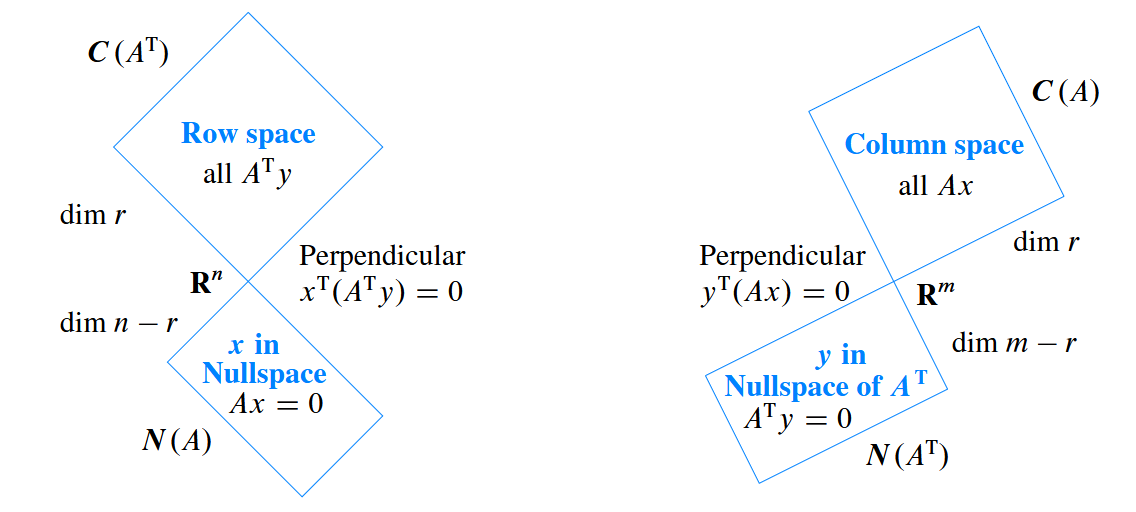
\includegraphics{figures/four_subspace.png}
\end{enumerate}

所谓零空间是使得列的线性组合为 0
的向量空间,而所谓左零空间实际上是使得行的线性组合为 0
的向量空间,参照上面对矩阵乘法的不同理解。

至于各个子空间是哪个维度空间的子空间实际上完全取决于其向量的长度。

对于向量空间,最重要的就是其基与维数,如何找到这些子空间的基与维数就是我们需要关注的。
下面的式子给出了关于矩阵 \(A\) 四个子空间所有的信息。 \[
E_{mm}A_{mn}= R = \begin{bmatrix} I_{r*r} & F_{r*(n-r)} \\
0_{(m-r)*r} & 0_{(m-r)*(n-r)} \\
\end{bmatrix}, rank = r
\]

\[
R_{m*n} N_{n*(n-r)} = 0
\]
需要注意的消元操作-行的初等变换,不改变行空间,但是会改变列空间------\((0, 1), (1, 0)\)
两个向量分别构成一维的空间,但是这两个空间是不同的!
\end{quote}

\(Ax = b\):

\[
x_\text{complete} = x_p + x_n, \text{其中} Ax_p = b, Ax_n = 0 \rightarrow A(x_p + x_n) = b
\]

\(x_p\) 为将所有自由变量赋值为 0 ,得到的特解,\(x_n\) 为 \(Ax = 0\) 为
\(A\) 的零空间的一般向量。

总结:

\begin{enumerate}
\def\labelenumi{\arabic{enumi}.}
\tightlist
\item
  若 \(r = m = n \rightarrow R = I\),
  即既没有多余的行,也没有多余的列,只有唯一解。
\item
  若 \(r = n < m \rightarrow R = \begin{bmatrix} I \\ 0 \end{bmatrix}\),
  有多余的行,无解或唯一解。
\item
  若 \(r = m < n \rightarrow R = \begin{bmatrix} I & F \end{bmatrix}\),
  即有多余的列,无穷多解。
\item
  若
  \(r < n, r < m \rightarrow R = \begin{bmatrix} I & F \\0 & 0 \\\end{bmatrix}\)
  , 即有多余的行与列,无解或者无穷多解。
\end{enumerate}

从上可以看出对于在2或者4的无解情形下,我们是无法解出线性方程组的;但是实际上对于情况2,我们可以通过将向量
\(b\) 投影到 \(A\)
的列空间之中得出一个最优解,而对于投影则涉及到正交的概念。

\begin{quote}
对于两个向量正交则
\(x^Ty = y^Tx = 0 \rightarrow ||x||^2 + ||y||^2 = ||x+y||^2\), 其中
\(||x||^2 = x^Tx\).
之前我们曾提到矩阵的四个子空间,实际上矩阵的行空间和它的零空间是互为正交补的,列空间与左零空间互为正交补。
\end{quote}

对于情形2无解的情况,要得到最优解,我们需要将 \(b\) 投影到 \(a/A\)
的方向,下面介绍如何进行投影。

考虑 向量 \(b\) 在 \(a\) 方向上投影的向量为 \(p\),既然其在 \(a\)
的方向上,则 \(p = ax\), 那么 \(e = b - p\) 则与 \(a\) 向量正交:

\[
a^T(b-p) = 0 \rightarrow a^T(b-xa) = 0 \rightarrow a^Tax = a^Tb
\]

解得 \(x = \frac{a^Tb}{a^Ta}, p = ax = a\frac{a^Tb}{a^Ta}\), 从 \(p\)
中我们可以分离出 矩阵 \(P = \frac{aa^T}{a^Ta}\),
该矩阵我们称之为投影矩阵,它将向量 \(b\) 投影到 \(a\) 的方向。

投影矩阵 \(P\)
是一个对称矩阵。显然,考虑到左乘一个矩阵为列的线性组合,投影矩阵既然是把
\(b\) 投影到 \(a\) 的方向,其显然和 \(a\)
有相同的列空间,其秩为1。另一方面,如果做两次投影则有
\(P^2b = Pb\),因为投影一次之后再投影,显然还是在原来的位置。因此矩阵
\(P\) 有如下性质:

\[
P^2 = P, P^T = P
\]

\begin{quote}
Gram-SChmidt 正交化

单位长度为 1, 并且彼此正交的向量称之为标准正交向量。如果矩阵 \(Q\)
的列向量为标准正交向量,则 \(Q^TQ = I\)
。一个标准正交的方正我们称之为``正交矩阵''(orthogonal matrix)。

从两个线性无关的向量开始 \(a\), \(b\)
开始其张成了一个空间,我们的目标就是找到一组标准正交的向量 \(q1, q2\)
能张成同样的空间。Schmidt提出如果有一组正交基 \(A\), \(B\),
那么我们令它们除以自己的长度就得到标准正交基。

\[
q_1 = \frac{A}{||A||}, q_2 = \frac{B}{||B||}
\]

Gram 提出了只要用向量 \(b\) 减去投影到 \(a\) 上的向量,即可得到一个与
\(a\) 垂直的向量,也就是上面提到的 \(e\) 的方向。

\[
B = \frac{aa^T}{a^Ta}b
\]

如果从三个线性无关的向量 \(a, b, c\) 出发,则可以通过从 \(c\) 中减去其在
\(a, b\) 向量上的投影得到与 \(a, b\) 垂直的向量 \(C\)。

\[
C = c - \frac{aa^Tc}{a^Ta} - \frac{bb^Tc}{b^Tb}
\]

施密特正交化的过程可以用矩阵运算的方式表示为 \(A = QR\), 此处 \(R\)
为上三角矩阵。

\[
\begin{bmatrix} a_1 & a_2 \end{bmatrix} = \begin{bmatrix} q_1 & q_2 \end{bmatrix} \begin{bmatrix} a_1^Tq_1 & a_2^Tq_1 \\ a_1^Tq_2 & a_2^Tq_2 \end{bmatrix}
\]

\(R\) 矩阵每个元素都是向量点积的值,而实际上点积代表的是 \(a\) 向量 在
\(q\) 向量上的投影长度与 \(q\) 的长度的乘积。如果 \(q\) 为 单位向量
则点积就是 \(a\) 在 \(q\) 方向的投影长度,如果 \(a\) 也为
单位向量,则点积就是两个向量夹角的余弦值。

结合右乘一个矩阵为列的线性组合,可以看到 \(R\) 矩阵每列的元素就是原每个
\(a\) 向量在 \(q\) 方向的投影长度,称之为权。
\end{quote}

将 \(b\) 向量投影到 \(A\) 矩阵的列空间, 则 \(p = Ax\)

\[
A^T(b - Ax) = 0 \rightarrow  A^TAx = A^Tb
\]

解得 \(x = (A^TA)^{-1}A^Tb, p = A(A^TA)^{-1}A^Tb\), 则投影矩阵
\(P = A(A^TA)^{-1}A^T\)

将向量 \(b\) 投影到列空间 \(A\) 与 投影到向量 \(a\)
的方向的一个特殊点在于,实际上 \(b\) 向量是在一个 \(m\)
空间之中,而之前提到是四个子空间,列空间与左零空间为正交补,为 \(m\)
维空间的子空间, 所以将 \(b\) 投影到 \(A\) 的列空间之中,实际是将 \(b\)
分解为两个向量,其中 \(p\) 向量在 \(A\) 列空间之中, 而 \(e\) 则在
左零空间之中,而将 \(b\) 投影到左零空间的矩阵为 \(I-P\)
为将其投影到左零空间的投影矩阵。

从 \(x\) 解的形式中,我们可以看到,用投影的方法求解线性方程组,需要
\(A^TA\) 存在逆矩阵,而其存在逆矩阵的条件就是 \(A\) 是列满秩的,
这就是该方法只能用于情形 2
无解的原因。应用投影矩阵求方程组最优解的方法,常用于``最小二乘法''拟合曲线。

\section{方阵 行列式 特征值
对角化}\label{ux65b9ux9635-ux884cux5217ux5f0f-ux7279ux5f81ux503c-ux5bf9ux89d2ux5316}

以下三个性质定义了行列式:

\begin{enumerate}
\def\labelenumi{\arabic{enumi}.}
\tightlist
\item
  \(det(I) = 1\)
\item
  如果交换行列式的两行,行列式的数值会反号。
\item
  \begin{enumerate}
  \def\labelenumii{\alph{enumii})}
  \tightlist
  \item
    如果矩阵某行乘以 \(t\), 则行列式的值要乘上
    \(t\)。b)行列式是``矩阵的行''的线性函数。
  \end{enumerate}
\end{enumerate}

从以上三个性质可以推导出下面七条性质:

\begin{enumerate}
\def\labelenumi{\arabic{enumi}.}
\setcounter{enumi}{3}
\tightlist
\item
  如果矩阵的两行完全相同,则它的行列式为 0。
\item
  从矩阵的某行 \(k\) 减去某一行 \(i\) 的倍数,并不改变行列式的数值。
\item
  如果矩阵 \(A\) 的某一行都是 0, 则其行列式为0。
\item
  三角阵行列式的值等于其对角线上数值(主元)的乘积。
\item
  当且仅当矩阵 \(A\) 为奇异矩阵时,其行列式为 0。
\item
  \(det(AB) = det(A)det(B)\).
\item
  \(det(A^T) = det(A)\).
\end{enumerate}

从性质 1,2, 3 可以推出行列式公式 (Formula for the determinant):

通过性质 3 对 \(n\) 阶矩阵进行拆分,我们可以得到所有只包含 \(n\)
个非零元素的行列式,对于二阶行列式,我们从一个拆分为两个,然后拆分为四个。对于三阶方阵,则从一个拆分成三个,然后拆分成九个,最后拆分为27个。然而,这些行列式中有很大一部分为
0。

每一个拆分出来的非 0
行列式都是再每行每列只有一个元素,就如同置换矩阵的元素分布,利用性质 3
可以将元素从行列式中提取出来,而置换矩阵的行列式值为 1, 或
-1,因此可以给出行列式公式;对于 \(n\) 阶方阵,其非 0 行列式的元素个数为
\(n!\)。

\[
det(A) = \sum_{n!}\pm{a_{1\alpha}a_{2\beta}...a_{n\omega}}
\]

将上面的行列式公式把某一行的元素提取,例如 \(a_{11}, a_{12}...\),
则每个元素的系数即为代数余子式,是一个低阶行列式的值,这个低阶行列式是由原矩阵去掉
\(a1j\) 所在行和列组成的。

对矩阵中的任意元素 \(a_{ij}\) 而言,其代数余子式 \(C_{ij}\)
就是矩阵的行列式的公式中 \(a_{ij}\) 的系数。\(C_{ij}\) 等于原矩阵移除第
\(i\) 行,第 \(j\) 列后剩余元素组成的 \(n - 1\) 矩阵的行列式数值乘以
\((-1)^{i + j}\)

对于 \(n\) 阶方阵,其行列式的代数余子式公式为:

\[
det(A) = a_{11}C_{11} + a_{12}C_{12} + \dots + a_{1n}C_{1n}
\]

然后实际上对于行列式的求解,消元法更简单高效。

将左乘一个矩阵看作对向量的变换,那么,如果一个变换不改变向量的方向,那么有:

\[
Ax = \lambda x
\]

上式的含义就是一个矩阵操作,只对一个向量进行放缩,如果矩上式存在非零解,那么

\[
det(A- \lambda I) = 0
\]

对于任意的 \(n \cdot n\) 矩阵,其具有 \(n\)
个特征值(可能存在重复的特征值),其和等于矩阵对角线元素之和,称为迹。其乘积等于矩阵的行列式。

对于对称矩阵而言,其永远具有实数的特征值,并且其特征向量正交;而对于反对称矩阵而言,具有纯虚数的特征值。

如果矩阵 \(A\) 具有 \(n\)
个线性无关的的特征向量,将它们作为列向量可以组成一个可逆方阵 \(S\),
并且有:

\[
\begin{align}
A\mathbf{S} &=  A \begin{bmatrix} \mathbf{x}_1 & \mathbf{x}_2 & \dots & \mathbf{x}_n \end{bmatrix} \\
   &= \begin{bmatrix} \lambda_1\mathbf{x}_1 & \lambda_2\mathbf{x}_2 &  \dots & \lambda_n\mathbf{x}_n \end{bmatrix}\\
   & = \begin{bmatrix} 
        \lambda_1 & 0         & \dots  & 0         \\
        0         & \lambda_2 &        & 0         \\ 
        \vdots    &           & \ddots & \vdots    \\
        0         & \dots     & 0      & \lambda_n  
       \end{bmatrix}  \\
  &= \mathbf{S} \Lambda
\end{align}
\]

那么有:

\[
A = S \Lambda S^{-1}
\]

特征值给矩阵的幂计算提供了方法。

如果 \(A\mathbf{x} = \lambda\mathbf{x}\), 则有
\(A^2\mathbf{x} = \lambda A\mathbf{x} = \lambda^2\mathbf{x}\), 说明矩阵
\(A^2\) 有着和 \(A\) 一样的特征向量,而特征值为
\(\lambda^2\)。写成对角化的形式则有:
\(A^2 = S\Lambda S^{-1} S\Lambda S^{-1}\)。同样的处理可以得到
\(A^{k} = S\Lambda^{k}S^{-1}\)。这说明 \(A^k\) 和 \(A\)
有相同的特征向量,而特征值为 \(\lambda^{k}\)。



\end{document}
